% Options for packages loaded elsewhere
\PassOptionsToPackage{unicode}{hyperref}
\PassOptionsToPackage{hyphens}{url}
%
\documentclass[
]{article}
\usepackage{amsmath,amssymb}
\usepackage{lmodern}
\usepackage{ifxetex,ifluatex}
\ifnum 0\ifxetex 1\fi\ifluatex 1\fi=0 % if pdftex
  \usepackage[T1]{fontenc}
  \usepackage[utf8]{inputenc}
  \usepackage{textcomp} % provide euro and other symbols
\else % if luatex or xetex
  \usepackage{unicode-math}
  \defaultfontfeatures{Scale=MatchLowercase}
  \defaultfontfeatures[\rmfamily]{Ligatures=TeX,Scale=1}
\fi
% Use upquote if available, for straight quotes in verbatim environments
\IfFileExists{upquote.sty}{\usepackage{upquote}}{}
\IfFileExists{microtype.sty}{% use microtype if available
  \usepackage[]{microtype}
  \UseMicrotypeSet[protrusion]{basicmath} % disable protrusion for tt fonts
}{}
\makeatletter
\@ifundefined{KOMAClassName}{% if non-KOMA class
  \IfFileExists{parskip.sty}{%
    \usepackage{parskip}
  }{% else
    \setlength{\parindent}{0pt}
    \setlength{\parskip}{6pt plus 2pt minus 1pt}}
}{% if KOMA class
  \KOMAoptions{parskip=half}}
\makeatother
\usepackage{xcolor}
\IfFileExists{xurl.sty}{\usepackage{xurl}}{} % add URL line breaks if available
\IfFileExists{bookmark.sty}{\usepackage{bookmark}}{\usepackage{hyperref}}
\hypersetup{
  pdftitle={Report Lucene},
  pdfauthor={Aarón Blanco Álvarez},
  hidelinks,
  pdfcreator={LaTeX via pandoc}}
\urlstyle{same} % disable monospaced font for URLs
\usepackage[margin=1in]{geometry}
\usepackage{color}
\usepackage{fancyvrb}
\newcommand{\VerbBar}{|}
\newcommand{\VERB}{\Verb[commandchars=\\\{\}]}
\DefineVerbatimEnvironment{Highlighting}{Verbatim}{commandchars=\\\{\}}
% Add ',fontsize=\small' for more characters per line
\usepackage{framed}
\definecolor{shadecolor}{RGB}{248,248,248}
\newenvironment{Shaded}{\begin{snugshade}}{\end{snugshade}}
\newcommand{\AlertTok}[1]{\textcolor[rgb]{0.94,0.16,0.16}{#1}}
\newcommand{\AnnotationTok}[1]{\textcolor[rgb]{0.56,0.35,0.01}{\textbf{\textit{#1}}}}
\newcommand{\AttributeTok}[1]{\textcolor[rgb]{0.77,0.63,0.00}{#1}}
\newcommand{\BaseNTok}[1]{\textcolor[rgb]{0.00,0.00,0.81}{#1}}
\newcommand{\BuiltInTok}[1]{#1}
\newcommand{\CharTok}[1]{\textcolor[rgb]{0.31,0.60,0.02}{#1}}
\newcommand{\CommentTok}[1]{\textcolor[rgb]{0.56,0.35,0.01}{\textit{#1}}}
\newcommand{\CommentVarTok}[1]{\textcolor[rgb]{0.56,0.35,0.01}{\textbf{\textit{#1}}}}
\newcommand{\ConstantTok}[1]{\textcolor[rgb]{0.00,0.00,0.00}{#1}}
\newcommand{\ControlFlowTok}[1]{\textcolor[rgb]{0.13,0.29,0.53}{\textbf{#1}}}
\newcommand{\DataTypeTok}[1]{\textcolor[rgb]{0.13,0.29,0.53}{#1}}
\newcommand{\DecValTok}[1]{\textcolor[rgb]{0.00,0.00,0.81}{#1}}
\newcommand{\DocumentationTok}[1]{\textcolor[rgb]{0.56,0.35,0.01}{\textbf{\textit{#1}}}}
\newcommand{\ErrorTok}[1]{\textcolor[rgb]{0.64,0.00,0.00}{\textbf{#1}}}
\newcommand{\ExtensionTok}[1]{#1}
\newcommand{\FloatTok}[1]{\textcolor[rgb]{0.00,0.00,0.81}{#1}}
\newcommand{\FunctionTok}[1]{\textcolor[rgb]{0.00,0.00,0.00}{#1}}
\newcommand{\ImportTok}[1]{#1}
\newcommand{\InformationTok}[1]{\textcolor[rgb]{0.56,0.35,0.01}{\textbf{\textit{#1}}}}
\newcommand{\KeywordTok}[1]{\textcolor[rgb]{0.13,0.29,0.53}{\textbf{#1}}}
\newcommand{\NormalTok}[1]{#1}
\newcommand{\OperatorTok}[1]{\textcolor[rgb]{0.81,0.36,0.00}{\textbf{#1}}}
\newcommand{\OtherTok}[1]{\textcolor[rgb]{0.56,0.35,0.01}{#1}}
\newcommand{\PreprocessorTok}[1]{\textcolor[rgb]{0.56,0.35,0.01}{\textit{#1}}}
\newcommand{\RegionMarkerTok}[1]{#1}
\newcommand{\SpecialCharTok}[1]{\textcolor[rgb]{0.00,0.00,0.00}{#1}}
\newcommand{\SpecialStringTok}[1]{\textcolor[rgb]{0.31,0.60,0.02}{#1}}
\newcommand{\StringTok}[1]{\textcolor[rgb]{0.31,0.60,0.02}{#1}}
\newcommand{\VariableTok}[1]{\textcolor[rgb]{0.00,0.00,0.00}{#1}}
\newcommand{\VerbatimStringTok}[1]{\textcolor[rgb]{0.31,0.60,0.02}{#1}}
\newcommand{\WarningTok}[1]{\textcolor[rgb]{0.56,0.35,0.01}{\textbf{\textit{#1}}}}
\usepackage{graphicx}
\makeatletter
\def\maxwidth{\ifdim\Gin@nat@width>\linewidth\linewidth\else\Gin@nat@width\fi}
\def\maxheight{\ifdim\Gin@nat@height>\textheight\textheight\else\Gin@nat@height\fi}
\makeatother
% Scale images if necessary, so that they will not overflow the page
% margins by default, and it is still possible to overwrite the defaults
% using explicit options in \includegraphics[width, height, ...]{}
\setkeys{Gin}{width=\maxwidth,height=\maxheight,keepaspectratio}
% Set default figure placement to htbp
\makeatletter
\def\fps@figure{htbp}
\makeatother
\setlength{\emergencystretch}{3em} % prevent overfull lines
\providecommand{\tightlist}{%
  \setlength{\itemsep}{0pt}\setlength{\parskip}{0pt}}
\setcounter{secnumdepth}{-\maxdimen} % remove section numbering
\ifluatex
  \usepackage{selnolig}  % disable illegal ligatures
\fi

\title{Report Lucene}
\author{Aarón Blanco Álvarez}
\date{28/4/2021}

\begin{document}
\maketitle

\hypertarget{introduction}{%
\section{Introduction}\label{introduction}}

In this report we are going to discuss the evolution in the three
versions of Lucene. For this goal, we need tools to make the analysis
like R Studio, R, etc. With this approach, will get metrics of the
system in a clear way than other tools and also, R provide us the
possibility of make our own metrics.

\hypertarget{materials-and-methods}{%
\section{Materials and methods}\label{materials-and-methods}}

For our purpose, we need RStudio with R, the programming language
itself. Also, the data in csv from the execution of Sourcemeter.
Furthermore, we will install some packages to load csv among others.
Here is an example:

\begin{figure}
\centering
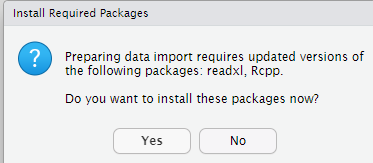
\includegraphics{EXCEL.png}
\caption{package instalation}
\end{figure}

\hypertarget{system-metrics}{%
\section{System Metrics}\label{system-metrics}}

Let us start with the main metrics, after import the excel, we will use
R to read the excels.

\hypertarget{method-hiding-factor-mhf-}{%
\subsection{(Method Hiding Factor
--MHF-)}\label{method-hiding-factor-mhf-}}

This is the proportion of hiding methods. Firstly, we have to read the
excels, we can do that with the \textbf{read.csv} instruction, after
that, we can save the columns need it in two variables. In this case, NM
and NPM. The meaning of this two variables are \emph{number of methods}
and \emph{number of public methods}.

As we can see, we can get private methods proportion if we make the
operation of divide number of public methods between all methods, then,
subtract to one. In theory, with each version, MHF is increasing, which
means that will be less bugs and technical debt, nevertheless, is very
small in this case.

\begin{Shaded}
\begin{Highlighting}[]
\NormalTok{luc49\_Class  }\OtherTok{\textless{}{-}} \FunctionTok{read.csv}\NormalTok{(}\StringTok{"Excel/Lucene4.9.0/luc49{-}Class.csv"}\NormalTok{) }
\NormalTok{luc491\_Class  }\OtherTok{\textless{}{-}} \FunctionTok{read.csv}\NormalTok{(}\StringTok{"Excel/Lucene4.9.1/luc491{-}Class.csv"}\NormalTok{) }
\NormalTok{luc41\_Class  }\OtherTok{\textless{}{-}} \FunctionTok{read.csv}\NormalTok{(}\StringTok{"Excel/Lucene4.10/luc410{-}Class.csv"}\NormalTok{) }

\NormalTok{NM }\OtherTok{\textless{}{-}}\NormalTok{ luc49\_Class[[}\StringTok{"NM"}\NormalTok{]];}
\NormalTok{NPM }\OtherTok{\textless{}{-}}\NormalTok{ luc49\_Class[[}\StringTok{"NPM"}\NormalTok{]];}
\NormalTok{Privado4}\FloatTok{.9} \OtherTok{\textless{}{-}}\NormalTok{ (}\DecValTok{1}\SpecialCharTok{{-}}\NormalTok{(}\FunctionTok{sum}\NormalTok{(NPM)}\SpecialCharTok{/}\FunctionTok{sum}\NormalTok{(NM)));}
\FunctionTok{print}\NormalTok{(Privado4}\FloatTok{.9}\NormalTok{);}
\end{Highlighting}
\end{Shaded}

\begin{verbatim}
## [1] 0.1861779
\end{verbatim}

\begin{Shaded}
\begin{Highlighting}[]
\NormalTok{NM }\OtherTok{\textless{}{-}}\NormalTok{ luc491\_Class[[}\StringTok{"NM"}\NormalTok{]];}
\NormalTok{NPM }\OtherTok{\textless{}{-}}\NormalTok{ luc491\_Class[[}\StringTok{"NPM"}\NormalTok{]];}
\NormalTok{Privado4.}\FloatTok{9.1} \OtherTok{\textless{}{-}}\NormalTok{ (}\DecValTok{1}\SpecialCharTok{{-}}\NormalTok{(}\FunctionTok{sum}\NormalTok{(NPM)}\SpecialCharTok{/}\FunctionTok{sum}\NormalTok{(NM)));}
\FunctionTok{print}\NormalTok{(Privado4.}\FloatTok{9.1}\NormalTok{);}
\end{Highlighting}
\end{Shaded}

\begin{verbatim}
## [1] 0.1843877
\end{verbatim}

\begin{Shaded}
\begin{Highlighting}[]
\NormalTok{NM }\OtherTok{\textless{}{-}}\NormalTok{ luc41\_Class[[}\StringTok{"NM"}\NormalTok{]];}
\NormalTok{NPM }\OtherTok{\textless{}{-}}\NormalTok{ luc41\_Class[[}\StringTok{"NPM"}\NormalTok{]];}
\NormalTok{Privado4}\FloatTok{.1} \OtherTok{\textless{}{-}}\NormalTok{ (}\DecValTok{1}\SpecialCharTok{{-}}\NormalTok{(}\FunctionTok{sum}\NormalTok{(NPM)}\SpecialCharTok{/}\FunctionTok{sum}\NormalTok{(NM)));}
\FunctionTok{print}\NormalTok{(Privado4}\FloatTok{.1}\NormalTok{);}
\end{Highlighting}
\end{Shaded}

\begin{verbatim}
## [1] 0.18451
\end{verbatim}

\hypertarget{attribute-hiding-factor-ahf-}{%
\subsection{(Attribute Hiding Factor
--AHF-)}\label{attribute-hiding-factor-ahf-}}

This is the proportion of hiding attributes. In this metric, we can make
the same as before but in this case, changing the number of methods for
attributes. So, we are working here with X43 (Number of attributes
column) and NPA, public attributes. The formula is almost the same,

\begin{Shaded}
\begin{Highlighting}[]
\NormalTok{NAtt }\OtherTok{\textless{}{-}}\NormalTok{ luc49\_Class[, }\DecValTok{43}\NormalTok{];}
\NormalTok{NPA }\OtherTok{\textless{}{-}}\NormalTok{ luc49\_Class[[}\StringTok{"NPA"}\NormalTok{]];}
\NormalTok{APrivado }\OtherTok{\textless{}{-}} \DecValTok{1}\SpecialCharTok{{-}}\NormalTok{(}\FunctionTok{sum}\NormalTok{(NPA)}\SpecialCharTok{/}\FunctionTok{sum}\NormalTok{(NAtt));}
\FunctionTok{print}\NormalTok{(APrivado);}
\end{Highlighting}
\end{Shaded}

\begin{verbatim}
## [1] 0.5661251
\end{verbatim}

\begin{Shaded}
\begin{Highlighting}[]
\NormalTok{NAtt }\OtherTok{\textless{}{-}}\NormalTok{ luc491\_Class[, }\DecValTok{43}\NormalTok{];}
\NormalTok{NPA }\OtherTok{\textless{}{-}}\NormalTok{ luc491\_Class[[}\StringTok{"NPA"}\NormalTok{]];}
\NormalTok{APrivado4.}\FloatTok{9.1} \OtherTok{\textless{}{-}} \DecValTok{1}\SpecialCharTok{{-}}\NormalTok{(}\FunctionTok{sum}\NormalTok{(NPA)}\SpecialCharTok{/}\FunctionTok{sum}\NormalTok{(NAtt));}
\FunctionTok{print}\NormalTok{(APrivado4.}\FloatTok{9.1}\NormalTok{);}
\end{Highlighting}
\end{Shaded}

\begin{verbatim}
## [1] 0.5661843
\end{verbatim}

\begin{Shaded}
\begin{Highlighting}[]
\NormalTok{NAtt }\OtherTok{\textless{}{-}}\NormalTok{ luc41\_Class[, }\DecValTok{43}\NormalTok{];}
\NormalTok{NPA }\OtherTok{\textless{}{-}}\NormalTok{ luc41\_Class[[}\StringTok{"NPA"}\NormalTok{]];}
\NormalTok{APrivado4\_1 }\OtherTok{\textless{}{-}}\NormalTok{ (}\DecValTok{1}\SpecialCharTok{{-}}\NormalTok{(}\FunctionTok{sum}\NormalTok{(NPA)}\SpecialCharTok{/}\FunctionTok{sum}\NormalTok{(NAtt)));}
\FunctionTok{print}\NormalTok{(APrivado4\_1);}
\end{Highlighting}
\end{Shaded}

\begin{verbatim}
## [1] 0.5661031
\end{verbatim}

\begin{Shaded}
\begin{Highlighting}[]
\CommentTok{\#Proporción de métodos heredados}
\CommentTok{\#(Method Inheritance Factor –MIF{-})}

\CommentTok{\#Leemos el dataset  }
\NormalTok{NM }\OtherTok{\textless{}{-}}\NormalTok{ luc49\_Class[[}\StringTok{"NM"}\NormalTok{]];}
\NormalTok{NLM }\OtherTok{\textless{}{-}}\NormalTok{ luc49\_Class[[}\StringTok{"NLM"}\NormalTok{]];}
\CommentTok{\#Calculamos el número de métodos heredados restando el número total de métodos al número de métodos publicos locales.}
\NormalTok{HEREADOS }\OtherTok{\textless{}{-}}\NormalTok{ (NM }\SpecialCharTok{{-}}\NormalTok{ NLM);}
\CommentTok{\#La proporción la hacemos mediante heredados dividos entre numero de métodos totales.}
\NormalTok{MIF }\OtherTok{\textless{}{-}}\NormalTok{ (}\FunctionTok{sum}\NormalTok{(HEREADOS)}\SpecialCharTok{/}\FunctionTok{sum}\NormalTok{(NM));}
\FunctionTok{print}\NormalTok{(MIF);}
\end{Highlighting}
\end{Shaded}

\begin{verbatim}
## [1] 0.8437718
\end{verbatim}

\begin{Shaded}
\begin{Highlighting}[]
\NormalTok{NM }\OtherTok{\textless{}{-}}\NormalTok{ luc491\_Class[[}\StringTok{"NM"}\NormalTok{]];}
\NormalTok{NLM }\OtherTok{\textless{}{-}}\NormalTok{ luc491\_Class[[}\StringTok{"NLM"}\NormalTok{]];}
\NormalTok{HEREADOS }\OtherTok{\textless{}{-}}\NormalTok{ (NM }\SpecialCharTok{{-}}\NormalTok{ NLM);}
\NormalTok{MIF4.}\FloatTok{9.1} \OtherTok{\textless{}{-}}\NormalTok{ (}\FunctionTok{sum}\NormalTok{(HEREADOS)}\SpecialCharTok{/}\FunctionTok{sum}\NormalTok{(NM));}
\FunctionTok{print}\NormalTok{(MIF4.}\FloatTok{9.1}\NormalTok{);}
\end{Highlighting}
\end{Shaded}

\begin{verbatim}
## [1] 0.8452233
\end{verbatim}

\begin{Shaded}
\begin{Highlighting}[]
\NormalTok{NM }\OtherTok{\textless{}{-}}\NormalTok{ luc41\_Class[[}\StringTok{"NM"}\NormalTok{]];}
\NormalTok{NLM }\OtherTok{\textless{}{-}}\NormalTok{ luc41\_Class[[}\StringTok{"NLM"}\NormalTok{]];}
\NormalTok{HEREADOS }\OtherTok{\textless{}{-}}\NormalTok{ (NM }\SpecialCharTok{{-}}\NormalTok{ NLM);}
\NormalTok{MIF4}\FloatTok{.1} \OtherTok{\textless{}{-}}\NormalTok{ (}\FunctionTok{sum}\NormalTok{(HEREADOS)}\SpecialCharTok{/}\FunctionTok{sum}\NormalTok{(NM));}
\FunctionTok{print}\NormalTok{(MIF4}\FloatTok{.1}\NormalTok{);}
\end{Highlighting}
\end{Shaded}

\begin{verbatim}
## [1] 0.8453527
\end{verbatim}

\begin{Shaded}
\begin{Highlighting}[]
\CommentTok{\#Proporción de atributos heredados.}
\CommentTok{\#(Attribute Inheritance Factor –AIF{-})}

\CommentTok{\#Leemos el dataset  }
\NormalTok{NAtt }\OtherTok{\textless{}{-}}\NormalTok{ luc49\_Class[[}\StringTok{"X43"}\NormalTok{]];}
\NormalTok{NLA }\OtherTok{\textless{}{-}}\NormalTok{ luc49\_Class[[}\StringTok{"NLA"}\NormalTok{]];}
\CommentTok{\#Calculamos el número de atributos heredados restando el número total de atributos al número de atributos publicos locales.}
\NormalTok{HEREADOS }\OtherTok{\textless{}{-}}\NormalTok{ (NAtt }\SpecialCharTok{{-}}\NormalTok{ NLA);}
\CommentTok{\#La proporción la hacemos mediante heredados dividos entre numero de atributos totales.}
\NormalTok{MIF }\OtherTok{\textless{}{-}}\NormalTok{ (}\FunctionTok{sum}\NormalTok{(HEREADOS)}\SpecialCharTok{/}\FunctionTok{sum}\NormalTok{(NAtt));}
\FunctionTok{print}\NormalTok{(MIF);}
\end{Highlighting}
\end{Shaded}

\begin{verbatim}
## [1] NaN
\end{verbatim}

\begin{Shaded}
\begin{Highlighting}[]
\NormalTok{NAtt }\OtherTok{\textless{}{-}}\NormalTok{ luc491\_Class[[}\StringTok{"X43"}\NormalTok{]];}
\NormalTok{NLA }\OtherTok{\textless{}{-}}\NormalTok{ luc491\_Class[[}\StringTok{"NLA"}\NormalTok{]];}
\NormalTok{HEREADOS }\OtherTok{\textless{}{-}}\NormalTok{ (NAtt }\SpecialCharTok{{-}}\NormalTok{ NLA);}
\NormalTok{MIF4.}\FloatTok{9.1} \OtherTok{\textless{}{-}}\NormalTok{ (}\FunctionTok{sum}\NormalTok{(HEREADOS)}\SpecialCharTok{/}\FunctionTok{sum}\NormalTok{(NAtt));}
\FunctionTok{print}\NormalTok{(MIF4.}\FloatTok{9.1}\NormalTok{);}
\end{Highlighting}
\end{Shaded}

\begin{verbatim}
## [1] NaN
\end{verbatim}

\begin{Shaded}
\begin{Highlighting}[]
\NormalTok{NAtt }\OtherTok{\textless{}{-}}\NormalTok{ luc41\_Class[[}\StringTok{"X43"}\NormalTok{]];}
\NormalTok{NLA }\OtherTok{\textless{}{-}}\NormalTok{ luc41\_Class[[}\StringTok{"NLA"}\NormalTok{]];}
\NormalTok{HEREADOS }\OtherTok{\textless{}{-}}\NormalTok{ (NAtt }\SpecialCharTok{{-}}\NormalTok{ NLA);}
\NormalTok{MIF4}\FloatTok{.1} \OtherTok{\textless{}{-}}\NormalTok{ (}\FunctionTok{sum}\NormalTok{(HEREADOS)}\SpecialCharTok{/}\FunctionTok{sum}\NormalTok{(NAtt));}
\FunctionTok{print}\NormalTok{(MIF4}\FloatTok{.1}\NormalTok{);}
\end{Highlighting}
\end{Shaded}

\begin{verbatim}
## [1] NaN
\end{verbatim}

\begin{Shaded}
\begin{Highlighting}[]
\CommentTok{\#Proporción de polimorfismo.}
\CommentTok{\#Polymorphism Factor (PF)}
\end{Highlighting}
\end{Shaded}

\begin{Shaded}
\begin{Highlighting}[]
\CommentTok{\#Proporción de acoplamiento.}
\CommentTok{\#(Coupling Factor –CF{-})}


\CommentTok{\# Acomplamiento y numero de ancestros}
\NormalTok{CBO }\OtherTok{\textless{}{-}}\NormalTok{ luc49\_Class[[}\StringTok{"CBO"}\NormalTok{]];}
\NormalTok{NOA }\OtherTok{\textless{}{-}}\NormalTok{ luc49\_Class[[}\StringTok{"NOA"}\NormalTok{]];}
\NormalTok{numeroClases }\OtherTok{\textless{}{-}} \FunctionTok{length}\NormalTok{(luc49\_Class[[}\StringTok{"ID"}\NormalTok{]]);}
\NormalTok{NumR }\OtherTok{\textless{}{-}}\NormalTok{ CBO}\SpecialCharTok{{-}}\NormalTok{NOA;}
\NormalTok{CF }\OtherTok{\textless{}{-}}\NormalTok{ (numeroClases }\SpecialCharTok{{-}} \DecValTok{1}\NormalTok{)}\SpecialCharTok{/}\FunctionTok{sum}\NormalTok{(NumR);}
\FunctionTok{print}\NormalTok{(CF);}
\end{Highlighting}
\end{Shaded}

\begin{verbatim}
## [1] 0.192708
\end{verbatim}

\begin{Shaded}
\begin{Highlighting}[]
\NormalTok{CBO }\OtherTok{\textless{}{-}}\NormalTok{ luc491\_Class[[}\StringTok{"CBO"}\NormalTok{]];}
\NormalTok{NOA }\OtherTok{\textless{}{-}}\NormalTok{ luc491\_Class[[}\StringTok{"NOA"}\NormalTok{]];}
\NormalTok{numeroClases }\OtherTok{\textless{}{-}} \FunctionTok{length}\NormalTok{(luc491\_Class[[}\StringTok{"ID"}\NormalTok{]]);}
\NormalTok{NumR }\OtherTok{\textless{}{-}}\NormalTok{ CBO}\SpecialCharTok{{-}}\NormalTok{NOA;}
\NormalTok{CF }\OtherTok{\textless{}{-}}\NormalTok{ (numeroClases }\SpecialCharTok{{-}} \DecValTok{1}\NormalTok{)}\SpecialCharTok{/}\FunctionTok{sum}\NormalTok{(NumR);}
\FunctionTok{print}\NormalTok{(CF);}
\end{Highlighting}
\end{Shaded}

\begin{verbatim}
## [1] 0.1926064
\end{verbatim}

\begin{Shaded}
\begin{Highlighting}[]
\NormalTok{CBO }\OtherTok{\textless{}{-}}\NormalTok{ luc41\_Class[[}\StringTok{"CBO"}\NormalTok{]];}
\NormalTok{NOA }\OtherTok{\textless{}{-}}\NormalTok{ luc41\_Class[[}\StringTok{"NOA"}\NormalTok{]];}
\NormalTok{numeroClases }\OtherTok{\textless{}{-}} \FunctionTok{length}\NormalTok{(luc41\_Class[[}\StringTok{"ID"}\NormalTok{]]);}
\NormalTok{NumR }\OtherTok{\textless{}{-}}\NormalTok{ CBO}\SpecialCharTok{{-}}\NormalTok{NOA;}
\NormalTok{CF }\OtherTok{\textless{}{-}}\NormalTok{ (numeroClases }\SpecialCharTok{{-}} \DecValTok{1}\NormalTok{)}\SpecialCharTok{/}\FunctionTok{sum}\NormalTok{(NumR);}
\FunctionTok{print}\NormalTok{(CF);}
\end{Highlighting}
\end{Shaded}

\begin{verbatim}
## [1] 0.1914854
\end{verbatim}

\begin{Shaded}
\begin{Highlighting}[]
\CommentTok{\#Metricas personales.}

\CommentTok{\#}
\end{Highlighting}
\end{Shaded}


\end{document}
